\section{Methodology}
\label{sec:methodology}

We evaluate a unified validated-memory framework across three final audited settings with different transfer structure.

% ----------------------------------------------------------------------------
\subsection{Environments}
\label{sec:environments}

\paragraph{ALFWorld.}
ALFWorld~\cite{shridhar2021alfworld} provides a text-based interface to the ALFRED embodied household benchmark. Agents issue actions from a fixed grammar of ${\sim}$15 verb templates (e.g., \texttt{go to}, \texttt{take}, \texttt{open}, \texttt{heat}). Six task types share a compositional goal structure: \textsc{Search} $\rightarrow$ \textsc{Acquire} $\rightarrow$ \textsc{Transform} $\rightarrow$ \textsc{Place}. The small object vocabulary (${\sim}$50 types) and shared sub-goal phases yield high structural overlap between tasks.

\paragraph{SQL.}
The SQL setting asks agents to produce executable queries for held-out database tasks.
It has a regular symbolic action language and many reusable syntactic patterns, but individual memories often have narrow transfer radius: a useful query correction can depend on local schema names, joins, or predicate choices that do not recur broadly.

\paragraph{ScienceWorld.}
ScienceWorld~\cite{wang2022scienceworld} contains science-themed interactive tasks spanning 30 categories.
It exposes reusable procedural motifs, but the final KB contains only one train variation per category and the retrieval/validation signal is noisy relative to the diversity of held-out tasks.
We therefore treat it as a diagnostic boundary case rather than as a positive transfer result.

% ----------------------------------------------------------------------------
\subsection{Base Agent: ReAct}
\label{sec:react}

All agents build on ReAct~\cite{yao2023react}, interleaving reasoning traces with actions. We use Gemini 2.5 Flash as the base LLM for all experiments.

% ----------------------------------------------------------------------------
\subsection{Memory Systems}
\label{sec:memory-systems}

Our framework augments ReAct with a persistent knowledge base and two retrieval mechanisms: proactive \emph{Context Retrieval} (CR) at task start and on-demand \emph{Tool Retrieval} (TR) during execution. We emphasize that Context Retrieval (CR) and Tool Retrieval (TR) address complementary aspects of transfer: CR supplies task-level guidance before acting, while TR enables action- or issue-level reuse when the agent asks for help. Their combination is designed to expose whether validated memories are useful before and during execution.

\begin{figure*}[t]
\centering
\begin{subfigure}[t]{0.48\textwidth}
    \centering
    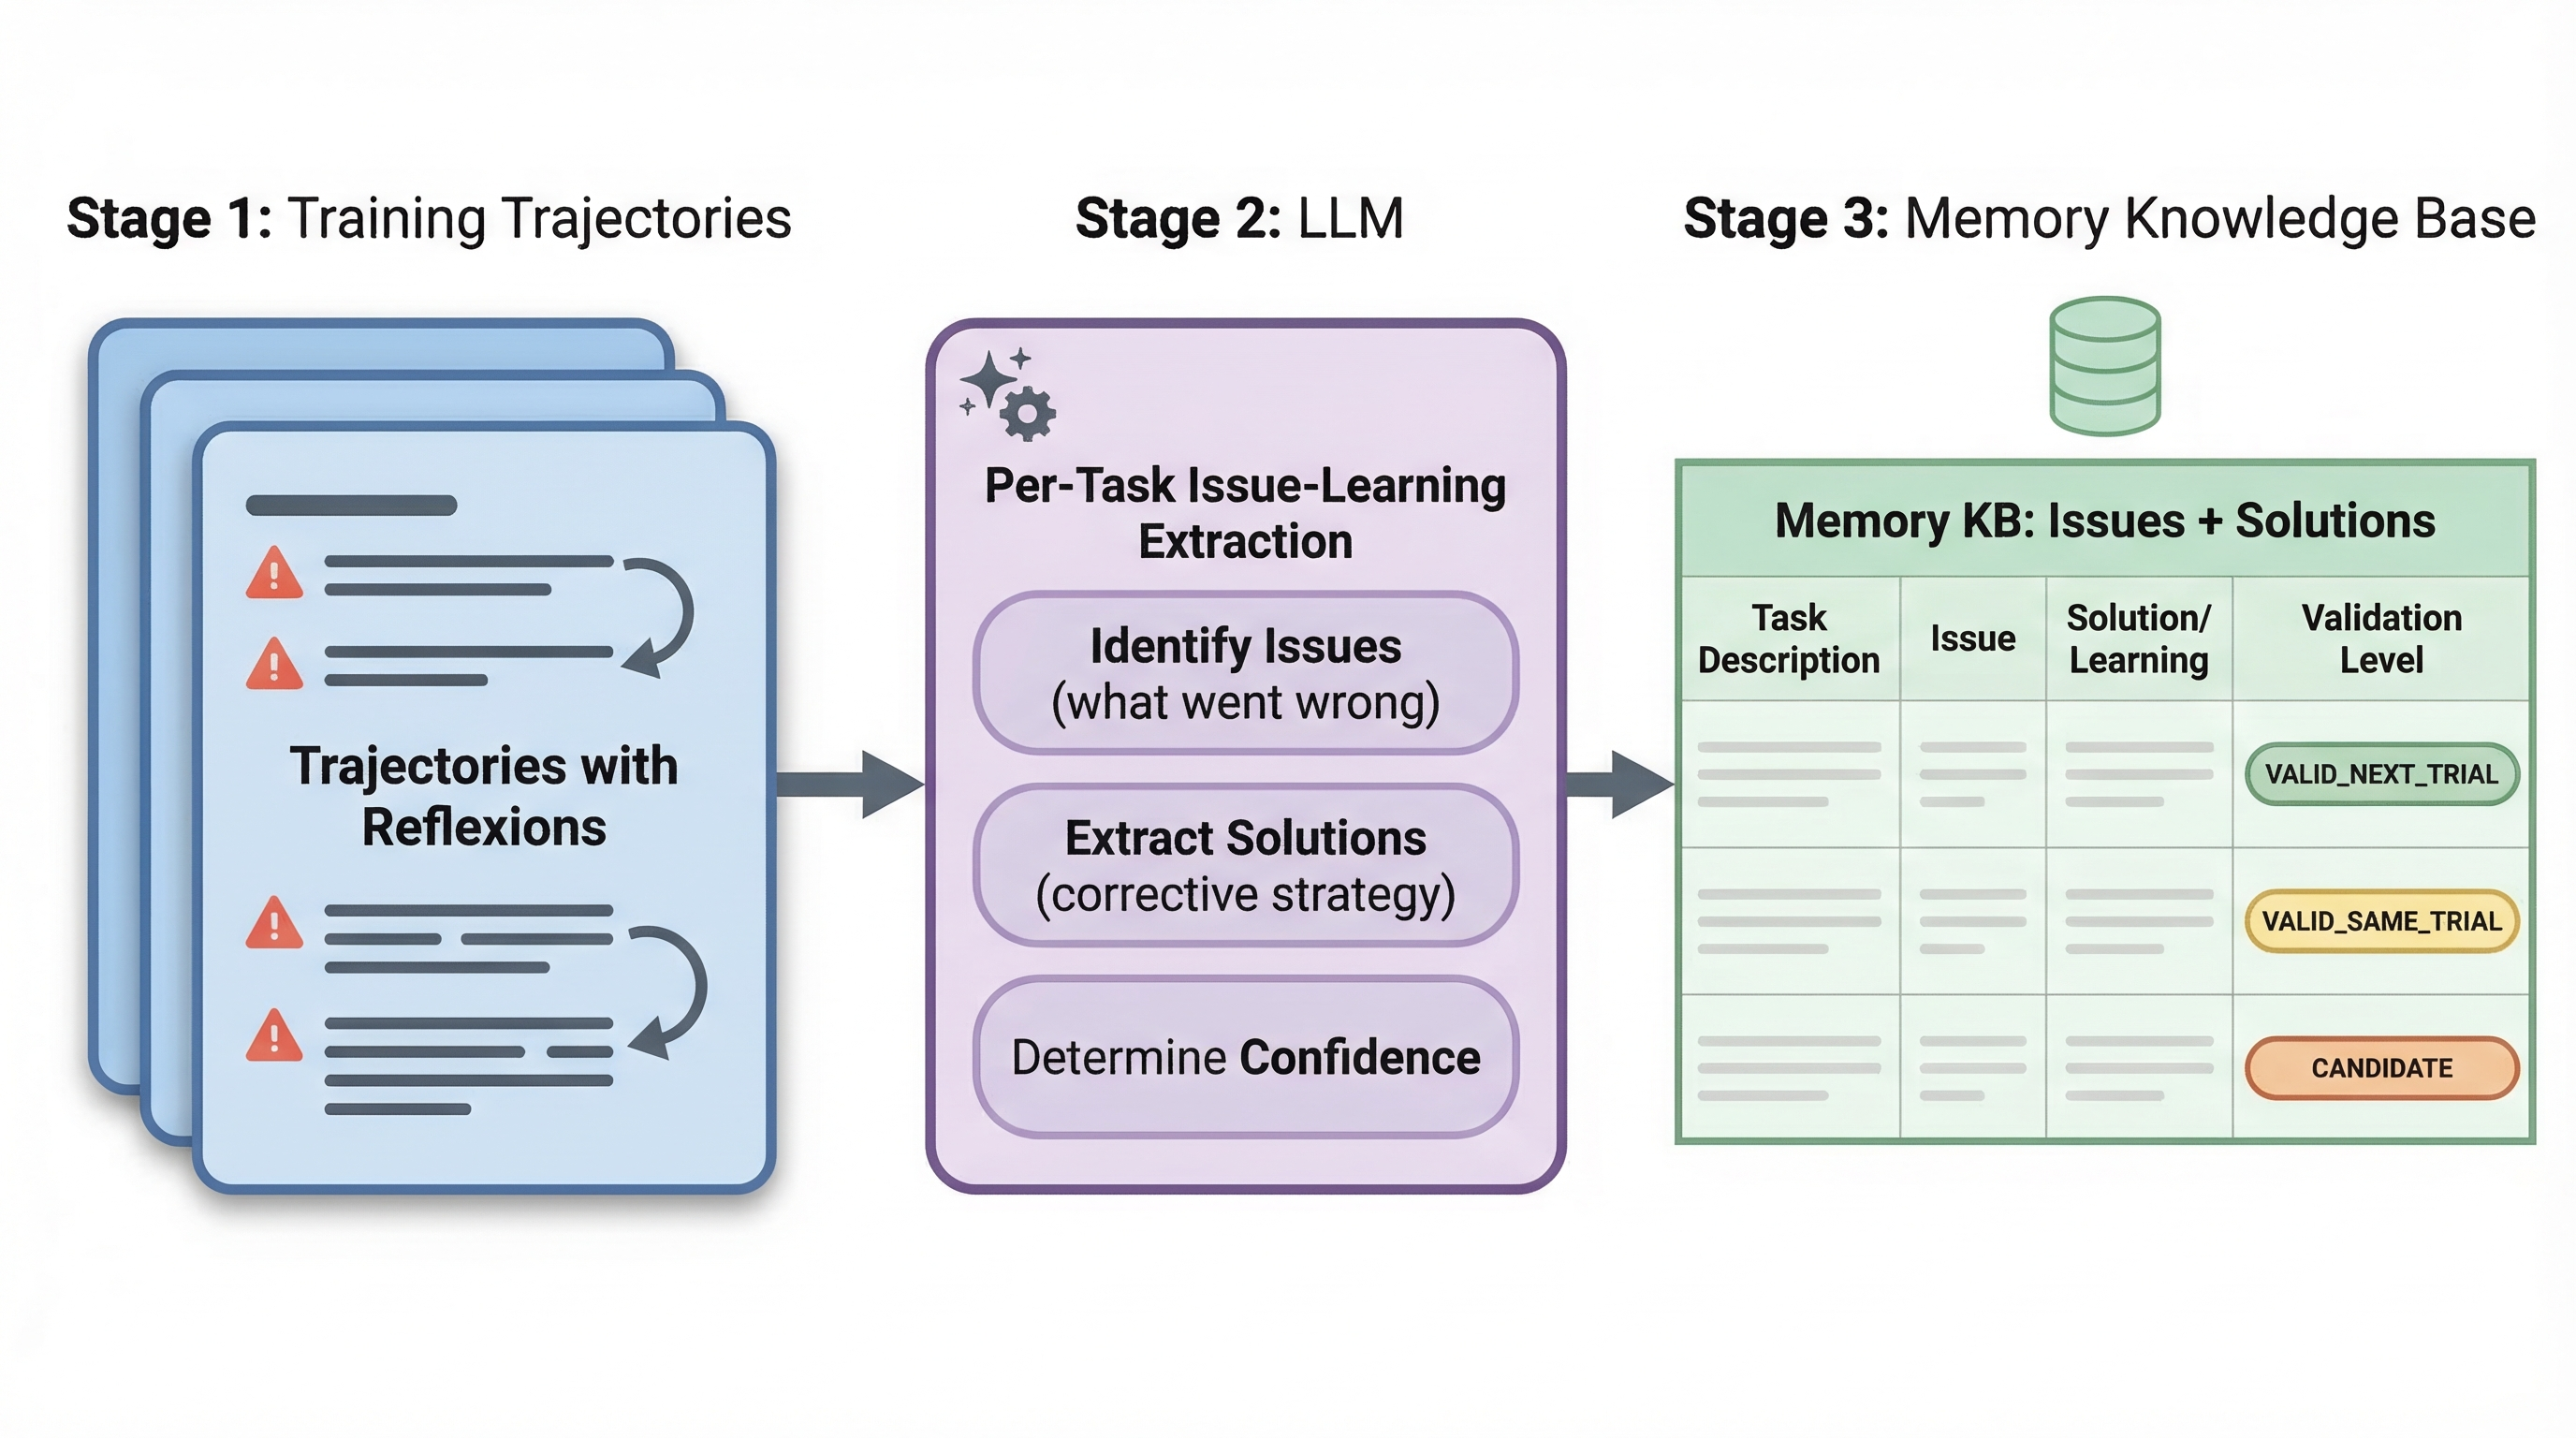
\includegraphics[width=\textwidth]{figures/section1_kb_generation.png}
    \caption{Offline KB construction from training trajectories.}
    \label{fig:kb-generation}
\end{subfigure}
\hfill
\begin{subfigure}[t]{0.48\textwidth}
    \centering
    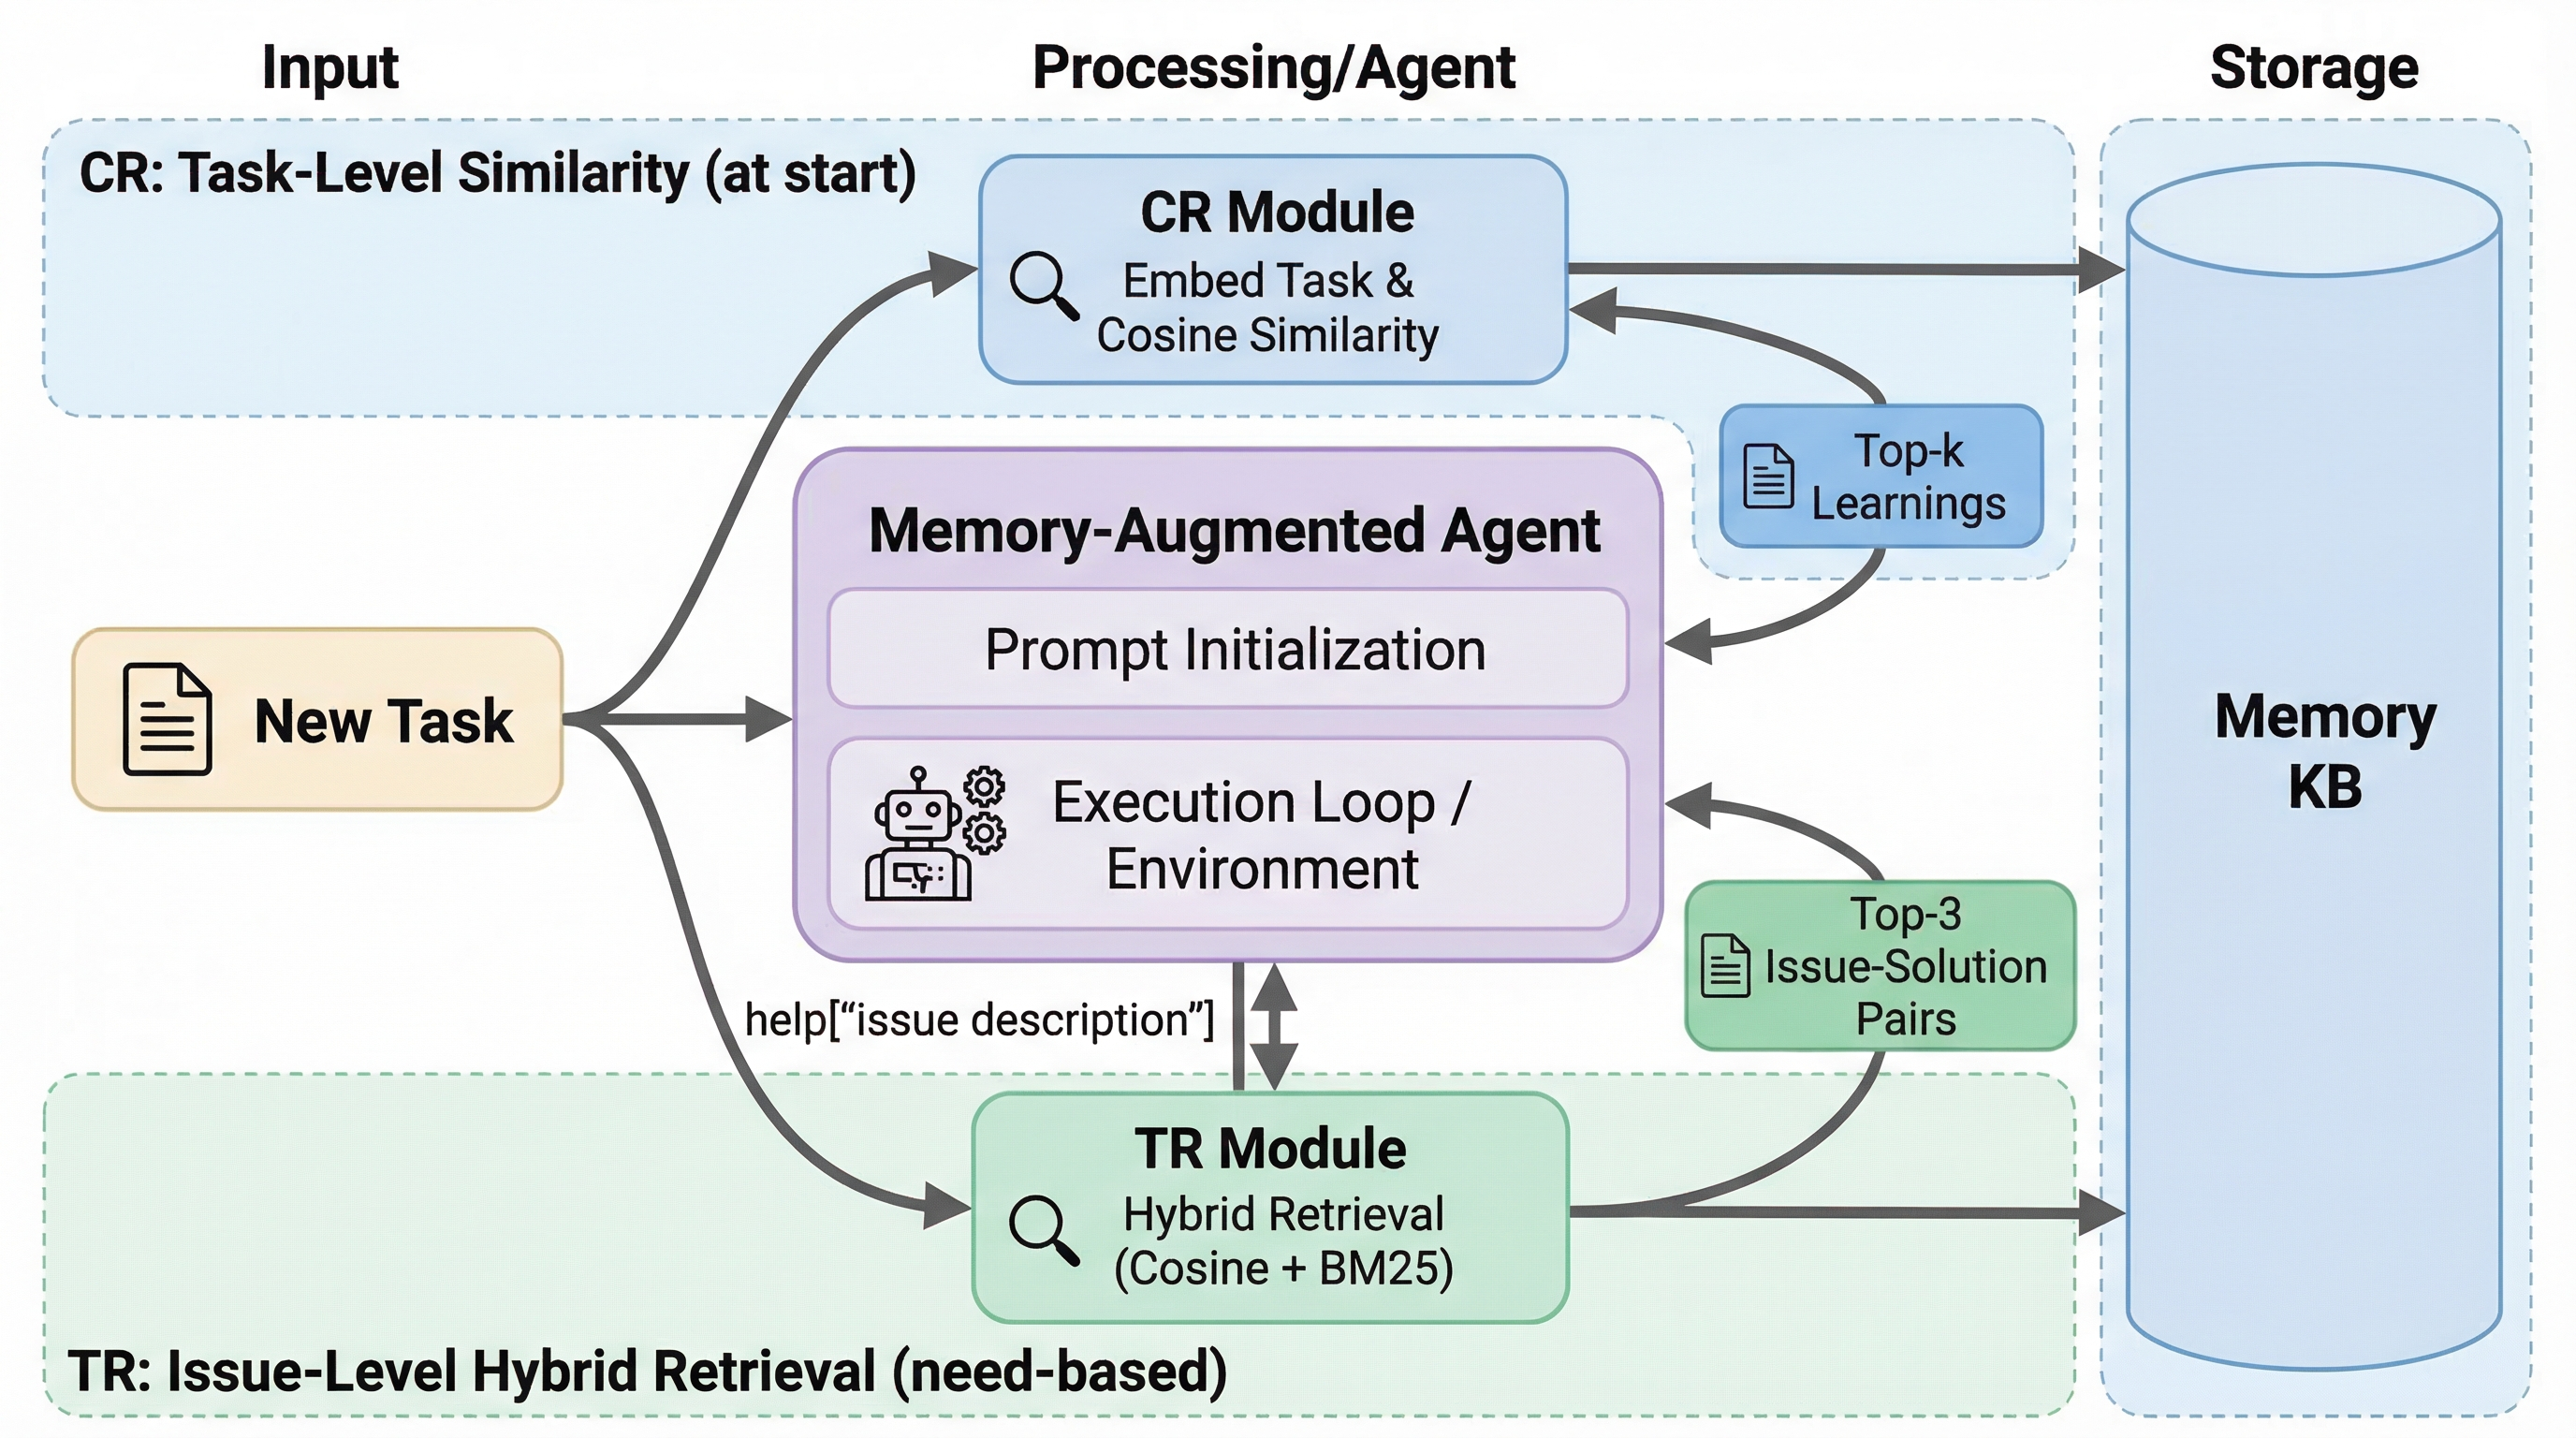
\includegraphics[width=\textwidth]{figures/section2_cr_tr_inference.png}
    \caption{Inference-time retrieval via CR and TR.}
    \label{fig:cr-tr-inference}
\end{subfigure}
\caption{Overview of the episodic memory framework. (a)~Training trajectories with reflexions are processed by an LLM to extract per-task issue--learning pairs with validation levels. (b)~Context Retrieval (CR) provides task-level learnings at the start; Tool Retrieval (TR) provides issue-level solutions on demand during execution.}
\label{fig:system-overview}
\end{figure*}

% ---- 3.3.1 ----
\subsubsection{Knowledge Base Construction}
\label{sec:kb-construction}

The knowledge base is constructed offline from training trajectories using LLM-based extraction. For each task, we extract \emph{issue--learning pairs}: structured records associating a mistake with its successful correction. Each entry includes task metadata, the issue--learning texts, a validation level reflecting downstream outcome (\textsc{Valid\_Next\_Trial}, \textsc{Valid\_Same\_Trial}, or \textsc{Candidate}), and provenance information. Final retrieval uses \textsc{Valid\_Next\_Trial} entries. We assign scalar validation weights $\omega$ to each level: $\omega_{\text{next}} = 1.0$, $\omega_{\text{same}} = 0.9$, $\omega_{\text{cand}} = 0.6$, used by both retrieval mechanisms to prioritize high-confidence learnings in the general algorithm. Full schema details are in Appendix~\ref{app:kb-schema}.

% ---- 3.3.2 ----
\subsubsection{Context Retrieval (CR)}
\label{sec:context-retrieval}

CR operates proactively: before the agent acts, it retrieves relevant past learnings based on embedding similarity (using \texttt{gemini-embedding-001}) between the new task description and historical tasks. The top-$k$ ($k{=}5$) most similar tasks are identified, their associated learnings are pooled and scored by:
\begin{equation}
    \text{Score}_{\text{CR}}(\ell) = \text{sim}(\mathbf{v}_q, \mathbf{v}_{t(\ell)}) \times \omega_{\ell}
\label{eq:cr-score}
\end{equation}
where $\text{sim}$ is cosine similarity and $\omega_{\ell}$ is the validation weight.

\paragraph{Dynamic context sizing.}
Rather than retrieving a fixed number of learnings, CR adapts the context window to neighborhood complexity. Let $L_{\max}$ denote the maximum learning count among the top-$k$ tasks. The retrieval quota is:
\begin{equation}
    N_{\text{pick}} = \min\!\left(\left\lceil \alpha \cdot L_{\max} \right\rceil,\; p\right)
\end{equation}
where $\alpha = 1.5$ is a scaling factor and $p \in [5, 25]$ is a tunable cap. The top-scored learnings are formatted as issue--learning pairs and prepended to the agent's prompt. The full procedure is given in Algorithm~\ref{alg:context-retrieval} (Appendix~\ref{app:algorithms}).

% ---- 3.3.3 ----
\subsubsection{Tool Retrieval (TR)}
\label{sec:tool-retrieval}

TR provides on-demand retrieval exposed as an action \texttt{help["issue"]}. It uses hybrid dense--sparse retrieval: cosine similarity over issue embeddings captures semantic matches, while BM25~\cite{robertson2009bm25} over concatenated fields captures lexical matches. The candidate pool is the union of the top-100 results from each strategy. Scores are normalized to $[0, 1]$ and fused:
\begin{equation}
    \text{Score}_{\text{TR}}(e) = \left(0.7 \cdot \text{cos}_{\text{norm}} + 0.3 \cdot \text{BM25}_{\text{norm}}\right) \times \omega_{e}
\label{eq:tr-score}
\end{equation}
The top-$k$ ($k{=}3$) results are returned as issue--solution pairs. The full procedure is given in Algorithm~\ref{alg:tool-retrieval} (Appendix~\ref{app:algorithms}).

% ---- 3.3.4 ----
\subsubsection{Hard Negative Control}
\label{sec:hard-neg}

To verify that gains stem from retrieval \emph{relevance} rather than additional prompt context, we introduce a hard negative control that inverts the selection criterion: CR retrieves the \emph{least} similar tasks and TR selects from the bottom of each retrieval strategy, producing prompts with the same number of learnings but from maximally irrelevant tasks.

% ----------------------------------------------------------------------------
\subsection{Reflexion for KB Construction}
\label{sec:reflexion}

We use Reflexion~\cite{shinn2023reflexion}, an iterative self-correction framework, to generate training trajectories for the trials7 knowledge bases. Unlike inference-time CR and TR, Reflexion is intra-task: it retries the same task with accumulated self-critiques. Our final held-out comparisons evaluate single-trial ReAct variants with and without retrieved cross-task memory.
